\chapter{\Stack}
\label{sec:stack}
\myindex{\Stack}

A pilha é uma das estruturas mais fundamentais na ciência da computação.
\footnote{\href{http://go.yurichev.com/17119}{wikipedia.org/wiki/Call\_stack}}.
\ac{AKA} \ac{LIFO}.

Tecnicamente, é só um bloco de memória junto com os registradores \ESP ou \RSP em x86 e x64, ou o \ac{SP} no ARM, como um ponteiro para aquele bloco.

\myindex{ARM!\Instructions!PUSH}
\myindex{ARM!\Instructions!POP}
\myindex{x86!\Instructions!PUSH}
\myindex{x86!\Instructions!POP}
As instruções mais frequente para o acesso da pilha são \PUSH e \POP (em ambos x86 e x64).
\PUSH subtrai de \ESP/\RSP/\ac{SP} 4 no modo 32-bits (ou 8 no modo 64-bits) e então escreve o conteúdo desse operando único para o endereço de memória apontado por \ESP/\RSP/\ac{SP}.

\POP é a operação reversa: recupera a informação da localização de memória que é apontada por \ac{SP}, 
carrega a mesma no operando da instrução (geralmente um registrador) e então adiciona 4 (ou 8) para o ponteiro da pilha.

Depois da alocação da pilha, o ponteiro aponta para o fundo da pilha.
\PUSH decrementa o ponteiro da pilha e \POP incrementa. O fundo da pilha está na verdade no começo do bloco de memória alocado para ela.
Pode parecer estranho, mas é a maneira como é feita.

ARM: \PTBRph{}

\section{Por que a pilha ``cresce'' para trás?}

Intuitivamente, nós podemos pensar que a pilha cresce para frente, em direção a endereços mais altos, como qualquer outra estrutura de informação.

O motivo da pilha crescer para trás é provavelmente histórico. Quando os computadores era grandes e ocupavam um cômodo todo, era mais fácil dividir a memória em duas partes, uma para a ‘heap’ e outra para a pilha.
Logicamente, era desconhecido o quão grande a heap e a pilha seriam durante a execução do programa, então essa solução era a mais simples possível.

\begin{center}
	\begin{tikzpicture}
	\tikzstyle{every path}=[thick]

	\node [rectangle,draw,minimum width=6cm, minimum height=2cm] (memory) {};
	\node [] [right=0.2cm of memory.west] (heap) {\MLHeap};
	\node [] [left=0.2cm of memory.east] (stack) {\MLStack};

	\node [] (center1) [right=2cm of memory.west] {};
	\node [] (center2) [left=2cm of memory.east] {};

	\draw [->] (heap) -- (center1);
	\draw [->] (stack) -- (center2);

	\node [] [above left=1.1cm and 0.2cm of heap] (t1) {\MLStartOfHeap};
	\node [] [above right=1.1cm and 0.2cm of stack] (t2) {\MLStartOfStack};

	\draw [->] (t1) -- (memory.west);
	\draw [->] (t2) -- (memory.east);

	\end{tikzpicture}
\end{center}


No \RitchieThompsonUNIX nós podemos ler:

\begin{framed}
\begin{quotation}
A parte relacionada ao usuário é dividida em três segmentos lógicos. O segmento de texto do programa começa na localização 0 no espaço virtual de endereçamento.
Durante a execução, esse segmento é protegido para não ser reescrito e uma única cópia dele é compartilhado entre
todos os processos executando o mesmo programa.
Começando no limite de 8Kbytes acima do segmento de texto do programa no espaço de endereçamento virtual começa um segmento de informação gravável,
não compartilhável e de um tamanho que pode ser extendido por uma chamada do sistema.
Começando no endereço mais alto no espaço de endereçamento virtual está a pilha, que automaticamente cresce para trás conforme o ponteiro da pilha do hardware se altera.
\end{quotation}
\end{framed}

Isso pode ser análogo a como um estudante escreve notas de duas matérias diferentes em um caderno só:
as notas para a primeira matéria são escritas como de costume e as notas para a segunda são escritas do final do caderno,
virando o mesmo. As anotações de uma matéria podem encontrar as da outra no meio, no caso de haver falta de espaço.

\section{Para que a pilha é usada?}

% subsections
\subsection{\RU{Сохранение адреса куда должно вернуться управление после вызова функции}
\EN{Save the return address where a function must return control after execution}}

\subsubsection{x86}

\index{x86!\Instructions!CALL}
\RU{При вызове другой функции через \CALL сначала в стек записывается адрес, указывающий на место аккурат после 
инструкции \CALL, затем делается безусловный переход (почти как \TT{JMP}) на адрес, указанный в операнде.} 
\EN{While calling another function with a \CALL instruction the address of the point exactly after the \CALL instruction is saved 
to the stack and then an unconditional jump to the address in the CALL operand is executed.} 

\index{x86!\Instructions!PUSH}
\index{x86!\Instructions!JMP}
\RU{\CALL ~--- это аналог пары инструкций \TT{PUSH address\_after\_call / JMP}}
\EN{The \CALL instruction is equivalent to a \TT{PUSH address\_after\_call / JMP operand} instruction pair}.

\index{x86!\Instructions!RET}
\index{x86!\Instructions!POP}
\RU{\RET вытаскивает из стека значение и передает управление по этому адресу ~--- 
это аналог пары инструкций \TT{POP tmp / JMP tmp}.}
\EN{\RET fetches a value from the stack and jumps to it~---it is equivalent to a \TT{POP tmp / JMP tmp} instruction pair.}

\index{\Stack!\RU{Переполнение стека}\EN{Stack overflow}}
\index{\Recursion}
\RU{Крайне легко устроить переполнение стека, запустив бесконечную рекурсию:}
\EN{Overflowing the stack is straightforward. Just run eternal recursion:}

\begin{lstlisting}
void f()
{
	f();
};
\end{lstlisting}

\RU{MSVC 2008 предупреждает о проблеме:}\EN{MSVC 2008 reports the problem:}

\begin{lstlisting}
c:\tmp6>cl ss.cpp /Fass.asm
Microsoft (R) 32-bit C/C++ Optimizing Compiler Version 15.00.21022.08 for 80x86
Copyright (C) Microsoft Corporation.  All rights reserved.

ss.cpp
c:\tmp6\ss.cpp(4) : warning C4717: 'f' : recursive on all control paths, function will cause runtime stack overflow
\end{lstlisting}

\dots \RU{но, тем не менее, создает нужный код}\EN{but generates the right code anyway}:

\begin{lstlisting}
?f@@YAXXZ PROC						; f
; File c:\tmp6\ss.cpp
; Line 2
	push	ebp
	mov	ebp, esp
; Line 3
	call	?f@@YAXXZ				; f
; Line 4
	pop	ebp
	ret	0
?f@@YAXXZ ENDP						; f
\end{lstlisting}

\dots \RU{причем, если включить оптимизацию (\Ox), то будет даже интереснее, без переполнения стека, 
но работать будет \IT{корректно}\footnote{здесь ирония}:}
\EN{Also if we turn on optimization (\Ox option) the optimized code will not overflow the stack 
but instead will work \IT{correctly}\footnote{irony here}:}

\begin{lstlisting}
?f@@YAXXZ PROC						; f
; File c:\tmp6\ss.cpp
; Line 2
$LL3@f:
; Line 3
	jmp	SHORT $LL3@f
?f@@YAXXZ ENDP						; f
\end{lstlisting}

\RU{GCC 4.4.1 генерирует точно такой же код в обоих случаях, хотя и не предупреждает о проблеме.}
\EN{GCC 4.4.1 generates similar code in both cases, although without issuing any warning about the problem.}

\subsubsection{ARM}

\index{ARM!\Registers!Link Register}
\RU{Программы для ARM также используют стек для сохранения \ac{RA}, куда нужно вернуться, но несколько иначе}\EN{ARM
programs also use the stack for saving return addresses, but differently}.
\RU{Как уже упоминалось в секции}\EN{As mentioned in} ``\HelloWorldSectionName''~(\ref{sec:hw_ARM}),
\RU{\ac{RA} записывается в регистр}\EN{the \ac{RA} is saved to the} \ac{LR} (\gls{link register}).
\RU{Но если есть необходимость вызывать какую-то другую функцию и использовать регистр \ac{LR} еще
раз, его значение желательно сохранить}
\EN{However, if one needs to call another function and use the \ac{LR} register
one more time its value should be saved}.
\index{Function prologue}
\RU{Обычно это происходит в прологе функции, часто мы видим там инструкцию вроде}
\EN{Usually it is saved in the function prologue. Often, we see instructions like}
\index{ARM!\Instructions!PUSH}
\index{ARM!\Instructions!POP}
\TT{``PUSH {R4-R7,LR}''} \RU{, а в эпилоге}\EN{along with this instruction in epilogue}
\TT{``POP {R4-R7,PC}''}\RU{ ~--- так сохраняются регистры, которые будут использоваться в текущей функции, в том числе}
\EN{~---thus register values
to be used in the function are saved in the stack, including} \ac{LR}.

\index{ARM!Leaf function}
\RU{Тем не менее, если некая функция не вызывает никаких более функций, в терминологии ARM она называется}
\EN{Nevertheless, if a function never calls any other function, in ARM terminology it is called a}
\IT{\gls{leaf function}}\footnote{\url{http://infocenter.arm.com/help/index.jsp?topic=/com.arm.doc.faqs/ka13785.html}}. 
\RU{Как следствие, ``leaf''-функция не сохраняет регистр \ac{LR} (потому что не изменяет его).}
\EN{As a consequence, leaf functions do not save the \ac{LR} register (because doesn't modify it).}
\RU{А если эта функция небольшая, использует мало регистров, она может не использовать стек вообще}
\EN{If this function is small and uses a small number of registers, it may not use the stack at all}.
\RU{Таким образом, в ARM возможен вызов небольших leaf-функций не используя стек}
\EN{Thus, it is possible to call leaf functions without using the stack}.
\RU{Это может быть быстрее чем в старых x86, ведь внешняя память для стека не используется}
\EN{This can be faster than on older x86 because external RAM is not used for the stack}
\footnote{\RU{Когда-то, очень давно, на PDP-11 и VAX на инструкцию CALL (вызов других функций) могло тратиться
вплоть до 50\% времени (возможно из-за работы с памятью),
поэтому считалось, что много небольших функций это \glslink{anti-pattern}{анти-паттерн}}
\EN{Some time ago, on PDP-11 and VAX, the CALL instruction (calling other functions) was expensive; up to 50\%
of execution time might be spent on it, so it was common sense that big number of small function is \gls{anti-pattern}}\cite[Chapter 4, Part II]{Raymond:2003:AUP:829549}.}.
\RU{Либо это может быть полезным для тех ситуаций, когда память для стека еще не выделена либо недоступна}
\EN{It can be useful for such situations when memory for the stack is not yet allocated or not available}.

\EN{Some examples of leaf functions here are}\RU{Некоторые примеры таких ф-ций здесь}: \listingname 
\ref{ARM_leaf_example1}, \ref{ARM_leaf_example2}, 
\ref{ARM_leaf_example3}, \ref{ARM_leaf_example4}, \ref{ARM_leaf_example5},
\ref{ARM_leaf_example6}, \ref{ARM_leaf_example7}, \ref{ARM_leaf_example10}.

\subsection{\RU{Передача параметров для функции}\EN{Passing function arguments}}

\RU{Самый распространенный способ передачи параметров в x86 называется}
\EN{The most popular way to pass parameters in x86 is called} ``cdecl'':

\begin{lstlisting}
push arg3
push arg2
push arg1
call f
add esp, 4*3
\end{lstlisting}

\RU{Вызываемая функция получает свои параметры также через указатель стека.}
\EN{\Gls{callee} functions get their arguments via the stack pointer.}

\RU{Следовательно, так будут расположены значения в стеке перед исполнением самой первой инструкции
ф-ции \ttf{}:}
\EN{Therefore, this is how the argument values will be located in the stack before the execution
of the \ttf{} function's very first instruction:}

\begin{center}
\begin{tabular}{ | l | l | }
\hline
ESP & \RU{адрес возврата}\EN{return address} \\
\hline
ESP+4 & \argument \#1, \MarkedInIDAAs{} \TT{arg\_0} \\
\hline
ESP+8 & \argument \#2, \MarkedInIDAAs{} \TT{arg\_4} \\
\hline
ESP+0xC & \argument \#3, \MarkedInIDAAs{} \TT{arg\_8} \\
\hline
\dots & \dots \\
\hline
\end{tabular}
\end{center}

\RU{См. также в соответствующем разделе о других способах передачи аргументов через стек}
\EN{For more information on other calling conventions see also section}~(\myref{sec:callingconventions}).
\RU{Важно отметить, что, в общем, никто не заставляет программистов передавать параметры именно через стек,
это не является требованием к исполняемому коду.}
\EN{It is worth noting that nothing obliges programmers to pass arguments through the stack. It is not a requirement.}
\RU{Вы можете делать это совершенно иначе, не используя стек вообще.}
\EN{One could implement any other method without using the stack at all.}

\RU{К примеру, можно выделять в \glslink{heap}{куче} место для аргументов, 
заполнять их и передавать в функцию указатель на это место через \EAX. И это вполне будет работать}
\EN{For example, it is possible to allocate a space for arguments in the \gls{heap}, fill it and pass it to a function 
via a pointer to this block in the \EAX register. This will work}
\footnote{\RU{Например, в книге Дональда Кнута ``Искусство программирования'', в разделе 1.4.1 
посвященном подпрограммам\cite[раздел 1.4.1]{Knuth:1998:ACP:521463}, 
мы можем прочитать о возможности располагать параметры для вызываемой подпрограммы после инструкции \JMP,
передающей управление подпрограмме. Кнут описывает что это было особенно удобно для компьютеров IBM System/360.}
\EN{For example, in the ``The Art of Computer Programming'' book by Donald Knuth, 
in section 1.4.1 dedicated to subroutines\cite[section 1.4.1]{Knuth:1998:ACP:521463},
we could read that one way to supply arguments to a subroutine is simply to list them after the \JMP instruction
passing control to subroutine. Knuth explains that this method was particularly convenient on IBM System/360.}}.
\RU{Однако, так традиционно сложилось, что в x86 и ARM передача аргументов происходит именно через стек.}
\EN{However, it is a convenient custom in x86 and ARM to use the stack for this purpose.} \\
\\
\RU{Кстати, вызываемая ф-ция не имеет информации, сколько аргументов было ей было передано.}
\EN{By the way, the \gls{callee} function does not have any information about how many arguments were passed.}
\RU{Функции Си с переменным количеством аргументов (как \printf) определяют их количество по 
спецификаторам строки формата (начинающиеся со знака \%).}
\EN{C functions with a variable number of arguments (like \printf) determine their number using format string  specifiers (which begin with the \% symbol).}
\RU{Если написать что-то вроде}\EN{If we write something like} 

\begin{lstlisting}
printf("%d %d %d", 1234);
\end{lstlisting}

\printf \RU{выведет 1234, затем еще два случайных числа, которые волею случая оказались в стеке рядом.}
\EN{will print 1234, and then two random numbers, which were laying next to it in the stack.}\\
\\
\RU{Вот почему не так уж и важно, как объявлять ф-цию \main}
\EN{That's why it is not very important how we declare the \main function}: \RU{как}\EN{as} \main, 
\TT{main(int argc, char *argv[])} 
\RU{либо}\EN{or} \TT{main(int argc, char *argv[], char *envp[])}.

\RU{В реальности, \ac{CRT}-код вызывает \main примерно так:}
\EN{In fact, the \ac{CRT}-code is calling \main roughly as:}

\begin{lstlisting}
push envp
push argv
push argc
call main
...
\end{lstlisting}

\RU{Если вы объявляете \main как \main без аргументов, они, тем не менее, присутствуют в стеке, но не используются.}
\EN{If you declare \main as \main without arguments, they are, nevertheless, still present in the stack, but
are not used.}
\RU{Если вы объявите \main как}\EN{If you declare \main as} \TT{main(int argc, char *argv[])}, 
\RU{вы будете использовать два аргумента, а третий останется для вашей ф-ции ``невидимым''.}
\EN{you will use two arguments, and the third will remain ``invisible'' for your function.}
\RU{Более того, можно даже объявить}\EN{Even further, it is possible to declare} \TT{main(int argc)}, 
\RU{и это будет работать}\EN{and it will work}.


\EN{\subsection{Local variable storage}

A function could allocate space in the stack for its local variables just by decreasing 
the \gls{stack pointer} towards the stack bottom.

% I think here, "stack bottom" means the lowest address in the stack space,
% but the reader might also think it means towards the top of the stack space,
% like in a pop, so you might change "towards the stack bottom" to
% "towards the lowest address of the stack", or just take it out,
% since "decreasing" also suggests that.

Hence, it's very fast, no matter how many local variables are defined.
It is also not a requirement to store local variables in the stack.
You could store local variables wherever you like, 
but traditionally this is how it's done.

}
\RU{\subsubsection{Хранение локальных переменных}

Функция может выделить для себя некоторое место в стеке для локальных переменных, просто отодвинув 
\glslink{stack pointer}{указатель стека} глубже к концу стека.

% I think here, "stack bottom" means the lowest address in the stack space,
% but the reader might also think it means towards the top of the stack space,
% like in a pop, so you might change "towards the stack bottom" to
% "towards the lowest address of the stack", or just take it out,
% since "decreasing" also suggests that.

Это очень быстро вне зависимости от количества локальных переменных.
Хранить локальные переменные в стеке не является необходимым требованием. 
Вы можете хранить локальные переменные где угодно. 
Но по традиции всё сложилось так.

}
\PTBR{\subsectionold{Armazenamento de variáveis locais}

Uma função poderia alocar espaço na pilha para suas variáveis locais simplesmente decrementando o ponteiro da pilha.

% I think here, "stack bottom" means the lowest address in the stack space,
% but the reader might also think it means towards the top of the stack space,
% like in a pop, so you might change "towards the stack bottom" to
% "towards the lowest address of the stack", or just take it out,
% since "decreasing" also suggests that.

Consequentemente, é muito rápido, não importando quantas variáveis locais serão definidas.
Também não é um requisito armazenar variáveis locais na pilha.
Você pode armazenar variáveis locais onde você quiser, mas, tradicionalmente, é assim que é feito.

}
\subsection{x86: \RU{Функция alloca()}\EN{alloca() function}}
\label{alloca}
\index{\CStandardLibrary!alloca()}
\RU{Интересен случай с функцией \TT{alloca()}}
\EN{It is worth noting the \TT{alloca()} function.}\footnote{
\RU{В MSVC, реализацию функции можно посмотреть в файлах}
\EN{In MSVC, the function implementation can be found in} 
  \TT{alloca16.asm} 
  \AndENRU 
  \TT{chkstk.asm} 
  \InENRU 
  \TT{C:\textbackslash{}Program Files (x86)\textbackslash{}Microsoft Visual Studio 10.0\textbackslash{}VC\textbackslash{}crt\textbackslash{}src\textbackslash{}intel}}. 

\RU{Эта функция работает как \TT{malloc()}, но выделяет память прямо в стеке.} 
\EN{This function works like \TT{malloc()} but allocates memory just on the stack.}

\RU{Память освобождать через \TT{free()} не нужно, так как эпилог функции~(\ref{sec:prologepilog})
вернет \ESP назад в изначальное состояние и выделенная память просто аннулируется.}
\EN{The allocated memory chunk does not need to be freed via a \TT{free()} function call, since the 
function epilogue~(\ref{sec:prologepilog}) will return \ESP back to its initial state and 
the allocated memory will be just annulled.} 

\RU{Интересна реализация функции \TT{alloca()}.}
\EN{It is worth noting how \TT{alloca()} is implemented.}

\RU{Эта функция, если упрощенно, просто сдвигает \ESP вглубь стека 
на столько байт, сколько вам нужно и возвращает \ESP в качестве указателя на выделенный блок.}
\EN{In simple terms, this function just shifts \ESP downwards toward the stack bottom by the number of bytes you 
need and sets \ESP as a pointer to the \IT{allocated} block.}
\RU{Попробуем:}\EN{Let's try:}

\lstinputlisting{patterns/02_stack/04_alloca/2_1.c}

\RU{(Функция \TT{\_snprintf()} работает так же, как и \printf, только вместо выдачи результата в 
\gls{stdout} (т.е., на терминал или в консоль),
записывает его в буфер \TT{buf}. \puts выдает содержимое буфера \TT{buf} в \gls{stdout}. Конечно, можно было бы
заменить оба этих вызова на один \printf, но мне нужно проиллюстрировать использование небольшого буфера.)}
\EN{(\TT{\_snprintf()} function works just like \printf, but instead of dumping the result into \gls{stdout} (e.g., to terminal or 
console), it writes to the \TT{buf} buffer. \puts copies \TT{buf} contents to \gls{stdout}. Of course, these two
function calls might be replaced by one \printf call, but I would like to illustrate small buffer usage.)}

\subsubsection{MSVC}

\RU{Компилируем}\EN{Let's compile} (MSVC 2010):

\lstinputlisting[caption=MSVC 2010]{patterns/02_stack/04_alloca/2_2_msvc.asm}

\index{Compiler intrinsic}
\RU {Единственный параметр в \TT{alloca()} передается через \EAX, а не как обычно через стек}
\EN{The sole \TT{alloca()} argument is passed via \EAX (instead of pushing into stack)}
\footnote{
\RU{Это потому, что alloca() ~--- это не сколько функция, сколько т.н. \IT{compiler intrinsic} (\ref{sec:compiler_intrinsic})}
\EN{It is because alloca() is rather compiler intrinsic (\ref{sec:compiler_intrinsic}) than usual function}.

\RU{Одна из причин, почему здесь нужна именно функция, а не несколько инструкций прямо в коде в том, что в реализации 
функции alloca() от \ac{MSVC}
есть также код, читающий из только что выделенной памяти, чтобы \ac{OS} подключила физическую память к этому региону \ac{VM}.}
\EN{One of the reason there is a separate function instead of couple instructions just in the code,
because \ac{MSVC} implementation
of the alloca() function also has a code, which reads from the memory just allocated, in order to let \ac{OS} to map
physical memory to this \ac{VM} region.}
}.
\RU{После вызова \TT{alloca()}, \ESP теперь указывает на блок в 600 байт, который 
мы можем использовать под \TT{buf}.}
\EN{After the \TT{alloca()} call, \ESP points to the block of 600 bytes and we can 
use it as memory for the \TT{buf} array.}

\subsubsection{GCC + \IntelSyntax}

\RU{А GCC 4.4.1 обходится без вызова других функций:}
\EN{GCC 4.4.1 can do the same without calling external functions:}

\lstinputlisting[caption=GCC 4.7.3]{patterns/02_stack/04_alloca/2_1_gcc_intel_O3.asm.\LANG}

\subsubsection{GCC + \ATTSyntax}

\RU{Посмотрим на тот же код, только в синтаксисе AT\&T}\EN{Let's see the same code, but in AT\&T syntax}:

\lstinputlisting[caption=GCC 4.7.3]{patterns/02_stack/04_alloca/2_1_gcc_ATT_O3.s}

\index{\ATTSyntax}
\RU{Всё то же самое, что и в прошлом листинге.}\EN{The code is the same as in the previous listing.}

\RU{Кстати}\EN{By the way}, \TT{movl \$3, 20(\%esp)} 
\RU{ ~--- это аналог}\EN{is analogous to} \TT{mov DWORD PTR [esp+20], 3} \RU{в Intel-синтаксисе:}
\EN{ in Intel-syntax}\RU{ при адресации памяти в виде}\EN{~---when addressing memory in form} \IT{\RU{регистр+смещение}\EN{register+offset}}, 
\RU{это записывается в AT\&T синтаксисе как}\EN{it is written as} 
\TT{\RU{смещение}\EN{offset}(\%\RU{регистр}\EN{register})}\EN{ in AT\&T syntax}.


\subsubsection{(Windows) SEH}
\myindex{Windows!Structured Exception Handling}

\ifdefined\RUSSIAN
В стеке хранятся записи \ac{SEH} для функции (если они присутствуют).
Читайте больше о нем здесь: (\myref{sec:SEH}).
\fi % RUSSIAN

\ifdefined\ENGLISH
\ac{SEH} records are also stored on the stack (if they are present).
Read more about it: (\myref{sec:SEH}).
\fi % ENGLISH

\ifdefined\BRAZILIAN
\ac{SEH} também são guardados na pilha (se estiverem presentes).
\PTBRph{}: (\myref{sec:SEH}).
\fi % BRAZILIAN

\ifdefined\ITALIAN
I record \ac{SEH}, se presenti, sono anch'essi memorizzati nello stack.
Maggiori informazioni qui: (\myref{sec:SEH}).
\fi % ITALIAN

\subsection{\RU{Защита от переполнений буфера}\EN{Buffer overflow protection}\PTBR{Proteção contra estouro de buffer}}

\RU{Здесь больше об этом}\EN{More about it here}\PTBR{Mais sobre aqui}~(\myref{subsec:bufferoverflow}).



\subsection{\PTBRph{}}

Talvez, o motivo para armazenar variáveis locais e registros SEH na pilha é que eles são desvinculados automaticamente depois do fim da função,
usando somente uma instrução para corrigir o ponteiro da pilha (geralmente é \ADD). Argumentos de funções, como podemos dizer, são
também desalocados automaticamente com o fim da função.
Como contraste, tudo armazenado na memória heap tem de ser desalocado explicitamente.

% sections
\EN{\section{A typical stack layout}

A typical stack layout in a 32-bit environment at the start of a function, 
before the first instruction execution looks like this:

\begin{center}
\begin{tabular}{ | l | l | }
\hline
\dots & \dots \\
\hline
ESP-0xC & \localVariable \#2, \MarkedInIDAAs{} \TT{var\_8} \\
\hline
ESP-8 & \localVariable \#1, \MarkedInIDAAs{} \TT{var\_4} \\
\hline
ESP-4 & \savedValueOf \EBP \\
\hline
ESP & \ReturnAddress \\
\hline
ESP+4 & \argument \#1, \MarkedInIDAAs{} \TT{arg\_0} \\
\hline
ESP+8 & \argument \#2, \MarkedInIDAAs{} \TT{arg\_4} \\
\hline
ESP+0xC & \argument \#3, \MarkedInIDAAs{} \TT{arg\_8} \\
\hline
\dots & \dots \\
\hline
\end{tabular}
\end{center}



% I think this only applies to RISC architectures
% that don't have a POP instruction that only lets you read one value
% (ie. ARM and MIPS).
% In x86, the return address is saved before entering the function,
% and the function does not have the chance to save the frame pointer.
% Also, you should mention that this is how the stack looks like
% right after the function prologue,
% which some readers might think is the first instruction,
% but is needed to save the frame pointer.
}
\RU{\section{Разметка типичного стека}

Разметка типичного стека в 32-битной среде
перед исполнением самой первой инструкции функции выглядит так:

\begin{center}
\begin{tabular}{ | l | l | }
\hline
\dots & \dots \\
\hline
ESP-0xC & \localVariable \#2, \MarkedInIDAAs{} \TT{var\_8} \\
\hline
ESP-8 & \localVariable \#1, \MarkedInIDAAs{} \TT{var\_4} \\
\hline
ESP-4 & \savedValueOf \EBP \\
\hline
ESP & \ReturnAddress \\
\hline
ESP+4 & \argument \#1, \MarkedInIDAAs{} \TT{arg\_0} \\
\hline
ESP+8 & \argument \#2, \MarkedInIDAAs{} \TT{arg\_4} \\
\hline
ESP+0xC & \argument \#3, \MarkedInIDAAs{} \TT{arg\_8} \\
\hline
\dots & \dots \\
\hline
\end{tabular}
\end{center}



% I think this only applies to RISC architectures
% that don't have a POP instruction that only lets you read one value
% (ie. ARM and MIPS).
% In x86, the return address is saved before entering the function,
% and the function does not have the chance to save the frame pointer.
% Also, you should mention that this is how the stack looks like
% right after the function prologue,
% which some readers might think is the first instruction,
% but is needed to save the frame pointer.

}
\PTBR{\section{Um modelo típico de pilha}

Um modelo típico de pilha em um ambiente 32-bits no início de uma função,
antes da execução da primeira instrução, se parece com isso:

\begin{center}
\begin{tabular}{ | l | l | }
\hline
\dots & \dots \\
\hline
ESP-0xC & \localVariable \#2, \MarkedInIDAAs{} \TT{var\_8} \\
\hline
ESP-8 & \localVariable \#1, \MarkedInIDAAs{} \TT{var\_4} \\
\hline
ESP-4 & \savedValueOf \EBP \\
\hline
ESP & \ReturnAddress \\
\hline
ESP+4 & \argument \#1, \MarkedInIDAAs{} \TT{arg\_0} \\
\hline
ESP+8 & \argument \#2, \MarkedInIDAAs{} \TT{arg\_4} \\
\hline
ESP+0xC & \argument \#3, \MarkedInIDAAs{} \TT{arg\_8} \\
\hline
\dots & \dots \\
\hline
\end{tabular}
\end{center}



% I think this only applies to RISC architectures
% that don't have a POP instruction that only lets you read one value
% (ie. ARM and MIPS).
% In x86, the return address is saved before entering the function,
% and the function does not have the chance to save the frame pointer.
% Also, you should mention that this is how the stack looks like
% right after the function prologue,
% which some readers might think is the first instruction,
% but is needed to save the frame pointer.
}
\section{\RU{Мусор в стеке}\EN{Noise in stack}}

\RU{Часто в этой книге я говорю о ``шуме'' или ``мусоре'' в стеке или памяти.}
\EN{Often in this book, I write about ``noise'' or ``garbage'' values in stack or memory.}
\RU{Откуда он берется}\EN{Where are they came from}?
\RU{Это то, что осталось там после исполнения предыдущих ф-ций.}
\EN{These are what was left in there after other function's executions.}
\RU{Короткий пример}\EN{Short example}:

\lstinputlisting{patterns/02_stack/08_noise/st.c}

\RU{Компилируем}\EN{Compiling}\dots

\lstinputlisting[caption=\NonOptimizing MSVC 2010]{patterns/02_stack/08_noise/st.asm}

\RU{Компилятор поворчит немного}\EN{The compiler will grumble for a little}\dots

\begin{lstlisting}
c:\Polygon\c>cl st.c /Fast.asm /MD
Microsoft (R) 32-bit C/C++ Optimizing Compiler Version 16.00.40219.01 for 80x86
Copyright (C) Microsoft Corporation.  All rights reserved.

st.c
c:\polygon\c\st.c(11) : warning C4700: uninitialized local variable 'c' used
c:\polygon\c\st.c(11) : warning C4700: uninitialized local variable 'b' used
c:\polygon\c\st.c(11) : warning C4700: uninitialized local variable 'a' used
Microsoft (R) Incremental Linker Version 10.00.40219.01
Copyright (C) Microsoft Corporation.  All rights reserved.

/out:st.exe
st.obj
\end{lstlisting}

\RU{Но когда я запускаю}\EN{But when I run}\dots

\begin{lstlisting}
c:\Polygon\c>st
1, 2, 3
\end{lstlisting}

\RU{Ох. Вот это странно. Мы ведь не устанавливали значения никаких переменных в}\EN{Oh. 
What a weird thing. We did not set any variables in} \TT{f2()}. 
\RU{Эти значения это ``приведения'', которые все еще в стеке.}
\EN{These are values are ``ghosts'', which are still in the stack.}

\clearpage
\RU{Загрузим пример в}\EN{Let's load the example into} \olly:

\begin{figure}[H]
\centering
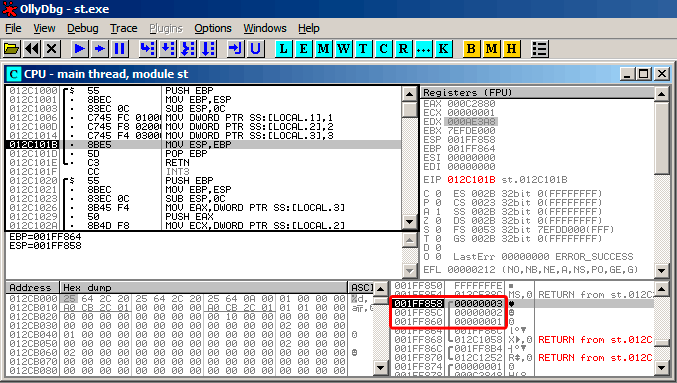
\includegraphics[scale=\FigScale]{patterns/02_stack/08_noise/olly1.png}
\caption{\olly: \TT{f1()}}
\label{fig:stack_noise_olly1}
\end{figure}

\RU{Когда}\EN{When} \TT{f1()} \RU{заполняет переменные}\EN{writes to} $a$, $b$ \AndENRU $c$ 
\RU{они сохранаяются по адресу}\EN{variables, they are stored at the address} \TT{0x14F85C} 
\RU{итд}\EN{and so on}.

\clearpage
\RU{А когда исполняется}\EN{And when} \TT{f2()}\EN{ executed}:

\begin{figure}[H]
\centering
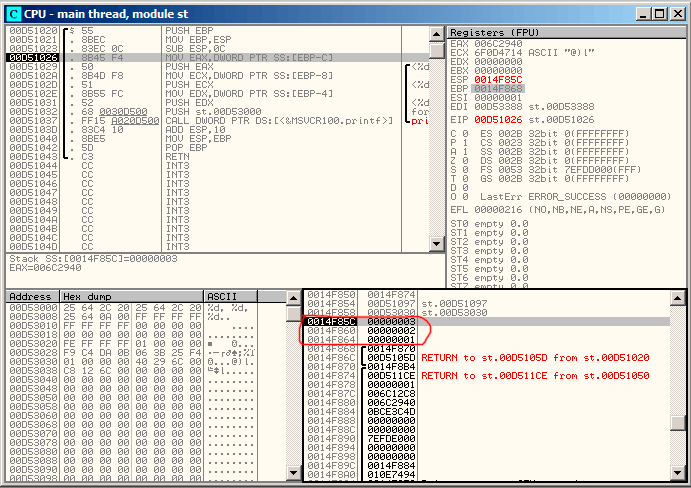
\includegraphics[scale=\FigScale]{patterns/02_stack/08_noise/olly2.png}
\caption{\olly: \TT{f2()}}
\label{fig:stack_noise_olly2}
\end{figure}

... $a$, $b$ \AndENRU $c$ \RU{в ф-ции}\EN{of} \TT{f2()} \RU{находятся по тем же адресам!}
\EN{are located at the same address!}
\RU{Пока никто не перезаписал их, так что они здесь в нетронутом виде.}
\EN{No one overwritten values yet, so they are still untouched here.}

\RU{Так что, для такой странной ситуации, несколько ф-ций должны исполняться друг за другом,
и \ac{SP} должен быть таким же при входе в ф-цию (т.е., у них должно быть равное кол-во
аргументов). Тогда, локальные переменные будут расположены в том же месте стека.}
\EN{So, for this weird situation, several functions should be called one after another and
\ac{SP} should be the same at each function entry (i.e., they should has same number
of arguments). Then, local variables will be located at the same point of stack.}

\RU{Подводя итоги, все значения в стеке (да и памяти вообще) это значения оставшиеся от 
исполнения предыдущих ф-ций}\EN{Summarizing, all values in stack (and memory cells at all) 
has values left there from previous function executions}.
\RU{Строго говоря, они не случайны, они скорее непредсказуемы}\EN{They are not 
random in strict sense, but rather has unpredictable values}.

\RU{А как иначе}\EN{How else}?
\RU{Вероятно, было бы возможным очищать части стека перед исполнением каждой ф-ции,
но это слишком много лишней (и ненужной) работы.}
\EN{Probably, it would be possible to clear stack portions before each function execution,
but that's too much extra (and needless) work.}

\section{\Exercises}

\begin{itemize}
	\item \url{http://challenges.re/51}
	\item \url{http://challenges.re/52}
\end{itemize}



